\documentclass[journal,12pt,twocolumn]{IEEEtran}
%
\usepackage{setspace}
\usepackage{gensymb}
\usepackage{xcolor}
\usepackage{caption}
%\usepackage{subcaption}
%\doublespacing
\singlespacing

%\usepackage{graphicx}
%\usepackage{amssymb}
%\usepackage{relsize}
\usepackage[cmex10]{amsmath}
\usepackage{mathtools}
%\usepackage{amsthm}
%\interdisplaylinepenalty=2500
%\savesymbol{iint}
%\usepackage{txfonts}
%\restoresymbol{TXF}{iint}
%\usepackage{wasysym}
\usepackage{amsthm}
\usepackage{enumerate}
\usepackage{mathrsfs}
\usepackage{txfonts}
\usepackage{stfloats}
\usepackage{cite}
\usepackage{cases}
\usepackage{subfig}
%       \usepackage[latin1]{inputenc}
       \usepackage{fullpage}
       \usepackage{color}
       \usepackage{array}
       \usepackage{calc}
       \usepackage{multirow}
       \usepackage{hhline}
       \usepackage{ifthen}


%\usepackage{xtab}
\usepackage{longtable}
\usepackage{multirow}
%\usepackage{algorithm}
%\usepackage{algpseudocode}
%\usepackage{enumitem}
\usepackage{mathtools}
\usepackage{iithtlc}
%\usepackage[framemethod=tikz]{mdframed}
\usepackage{listings}
\usepackage{tikz}

%\usepackage{stmaryrd}


%\usepackage{wasysym}
%\newcounter{MYtempeqncnt}
\DeclareMathOperator*{\Res}{Res}
%\renewcommand{\baselinestretch}{2}
\renewcommand\thesection{\arabic{section}}
\renewcommand\thesubsection{\thesection.\arabic{subsection}}
\renewcommand\thesubsubsection{\thesubsection.\arabic{subsubsection}}

\renewcommand\thesectiondis{\arabic{section}}
\renewcommand\thesubsectiondis{\thesectiondis.\arabic{subsection}}
\renewcommand\thesubsubsectiondis{\thesubsectiondis.\arabic{subsubsection}}

% correct bad hyphenation here
\hyphenation{op-tical net-works semi-conduc-tor}
\def\inputGnumericTable{}                                 %%
\lstset{
%language=Python,
frame=single, 
breaklines=true,
columns=fullflexible,
literate = {-}{-}1
}

%\lstset{
	%%basicstyle=\small\ttfamily\bfseries,
	%%numberstyle=\small\ttfamily,
	%language=Octave,
	%backgroundcolor=\color{white},
	%%frame=single,
	%%keywordstyle=\bfseries,
	%%breaklines=true,
	%%showstringspaces=false,
	%%xleftmargin=-10mm,
	%%aboveskip=-1mm,
	%%belowskip=0mm
%}

%\surroundwithmdframed[width=\columnwidth]{lstlisting}


\begin{document}
%

\theoremstyle{definition}
\newtheorem{theorem}{Theorem}[section]
\newtheorem{problem}{Problem}
\newtheorem{proposition}{Proposition}[section]
\newtheorem{lemma}{Lemma}[section]
\newtheorem{corollary}[theorem]{Corollary}
\newtheorem{example}{Example}[section]
\newtheorem{definition}{Definition}[section]
%\newtheorem{algorithm}{Algorithm}[section]
%\newtheorem{cor}{Corollary}
\newcommand{\BEQA}{\begin{eqnarray}}
\newcommand{\EEQA}{\end{eqnarray}}
\newcommand{\define}{\stackrel{\triangle}{=}}

\bibliographystyle{IEEEtran}
%\bibliographystyle{ieeetr}

\providecommand{\nCr}[2]{\,^{#1}C_{#2}} % nCr
\providecommand{\nPr}[2]{\,^{#1}P_{#2}} % nPr
\providecommand{\mbf}{\mathbf}
\providecommand{\pr}[1]{\ensuremath{\Pr\left(#1\right)}}
\providecommand{\qfunc}[1]{\ensuremath{Q\left(#1\right)}}
\providecommand{\sbrak}[1]{\ensuremath{{}\left[#1\right]}}
\providecommand{\lsbrak}[1]{\ensuremath{{}\left[#1\right.}}
\providecommand{\rsbrak}[1]{\ensuremath{{}\left.#1\right]}}
\providecommand{\brak}[1]{\ensuremath{\left(#1\right)}}
\providecommand{\lbrak}[1]{\ensuremath{\left(#1\right.}}
\providecommand{\rbrak}[1]{\ensuremath{\left.#1\right)}}
\providecommand{\cbrak}[1]{\ensuremath{\left\{#1\right\}}}
\providecommand{\lcbrak}[1]{\ensuremath{\left\{#1\right.}}
\providecommand{\rcbrak}[1]{\ensuremath{\left.#1\right\}}}
\theoremstyle{remark}
\newtheorem{rem}{Remark}
\newcommand{\sgn}{\mathop{\mathrm{sgn}}}
\providecommand{\abs}[1]{\left\vert#1\right\vert}
\providecommand{\res}[1]{\Res\displaylimits_{#1}} 
\providecommand{\norm}[1]{\lVert#1\rVert}
\providecommand{\mtx}[1]{\mathbf{#1}}
\providecommand{\mean}[1]{E\left[ #1 \right]}
\providecommand{\fourier}{\overset{\mathcal{F}}{ \rightleftharpoons}}
%\providecommand{\hilbert}{\overset{\mathcal{H}}{ \rightleftharpoons}}
\providecommand{\system}{\overset{\mathcal{H}}{ \longleftrightarrow}}
	%\newcommand{\solution}[2]{\textbf{Solution:}{#1}}
\newcommand{\solution}{\noindent \textbf{Solution: }}
\providecommand{\dec}[2]{\ensuremath{\overset{#1}{\underset{#2}{\gtrless}}}}
%\numberwithin{equation}{subsection}
\numberwithin{equation}{problem}
%\numberwithin{problem}{subsection}
%\numberwithin{definition}{subsection}
%\makeatletter
%\@addtoreset{figure}{problem}
%\makeatother
%
%\let\StandardTheFigure\thefigure
%%\renewcommand{\thefigure}{\theproblem.\arabic{figure}}
%\renewcommand{\thefigure}{\theproblem}


%\numberwithin{figure}{subsection}

\def\putbox#1#2#3{\makebox[0in][l]{\makebox[#1][l]{}\raisebox{\baselineskip}[0in][0in]{\raisebox{#2}[0in][0in]{#3}}}}
     \def\rightbox#1{\makebox[0in][r]{#1}}
     \def\centbox#1{\makebox[0in]{#1}}
     \def\topbox#1{\raisebox{-\baselineskip}[0in][0in]{#1}}
     \def\midbox#1{\raisebox{-0.5\baselineskip}[0in][0in]{#1}}

\vspace{3cm}

\title{
\logo{
Flashing STM32 using STLINK or RPI GPIO
}
}%
\author{Alok Ranjan Kesari and G. V. V. Sharma% 
%\author{Alok Ranjan Kesari$^{1}$ and Dr. G. V. V. Sharma$^{2}$% 
%\thanks{$^{1}$Alok Ranjan Kesari was an intern with the Department of Electrical Engineering, IIT Hyderabad
 %       {\tt\small alok.kesari@yahoo.co.in}}%
%\thanks{$^{2}$Dr. G. V. V. Sharma is with the Department of Electrical Engineering, IIT Hyderabad
%        {\tt\small gadepall@iith.ac.in}}%
\thanks{ The authors are with the Department of Electrical Engineering, IIT Hyderabad
        {\tt\small alok.kesari@yahoo.co.in, gadepall@iith.ac.in}}%

}



% make the title area
\maketitle

%\newpage

\tableofcontents


%%%%%%%%%%%%%%%%%%%%%%%%%%%%%%%%%%%%%%%%%%%%%%%%%%%%%%%%
\begin{abstract}
This manual shows how to program an STM32 board using STLINK and Raspberry Pi. The procedure is the same for any Linux machine.
\end{abstract}
\section{Components}
The necessary components for this manual are listed in Table \ref{table:components}.
\begin{table}[!h]
\centering
\input{./figs/components.tex}
\caption{}
\label{table:components}
\end{table}
%
\section{Software Setup}
Open a terminal and execute the following commands
\begin{lstlisting}
cd ~
mkdir -p ~/sandbox
cd ~/sandbox
\end{lstlisting}
\subsection{ Install Necessary Packages}
\begin{lstlisting}
sudo apt-get install git autoconf libtool make automake texinfo pkg-config libusb-1.0-0 libusb-1.0-0-dev gcc-arm-none-eabi libnewlib-arm-none-eabi telnet
\end{lstlisting}

\subsection{Installing Openocd and Programming Environment}
\begin{lstlisting}
git clone git://repo.or.cz/openocd.git
git clone https://github.com/gadepall/STM32F103C8T6.git
\end{lstlisting}
\subsection{Configure Openocd}
\begin{lstlisting}
cd openocd
./bootstrap 
./configure --enable-sysfsgpio --enable-bcm2835gpio
make
sudo make install
\end{lstlisting}
%
While using STLINK, \textbf{./configure} without the --enable switches is sufficient.
\section{Hardware Setup}
\subsection{STLINK}
Connect the STLINK to a USB port of the Raspberry Pi.  The hardware connections between the STLINK and STM32 are available in Table \ref{table:pins}. See Fig. \ref{fig:stm_black} as well for the {\em black pill}  board.  Fig. \ref{fig:stm_blue} shows the {\em blue pill} board.
\begin{table}[!h]
\centering
\input{./figs/pins.tex}
\caption{STLINK-STM32 connections}
\label{table:pins}
\end{table}
\subsection{RPI  GPIO}
On the RPi, type
\begin{lstlisting}
pinout
\end{lstlisting}
%
This will give the GPIO pin configuration on the RPi. Now open
\begin{lstlisting}
nano /usr/local/share/openocd/scripts/interface/sysfsgpio-raspberrypi.cfg
\end{lstlisting}
%
and verify that the file contains the lines (at different locations)
\begin{lstlisting}
# Each of the SWD lines need a gpio number set: swclk swdio
# Header pin numbers: 23 22
sysfsgpio_swd_nums 11 25

# Header pin numbers: TRST - 26, SRST - 18
sysfsgpio_srst_num 24
reset_config srst_only srst_push_pull
\end{lstlisting}
%
Note that the above configuration was obtained for an \textbf{RPi Zero W}. It may be different for other RPis.  Remove the \# before the  lines, if necessary.  These lines provide information on the pin connections between the Rpi and STM32 as shown in Table \ref{table:raspstm}.
\begin{table}[!h]
\centering
%\resizebox{0.52\columnwidth}{!}{%
\begin{tabular}{|c|c|}
\hline
\textbf{Raspberry Pi} & \textbf{STM32} \\ \hline
GND (Pin 6)           & GND            \\ \hline
3.3V (Pin 1)          & 3.3V           \\ \hline
GPIO 25 (Pin 22)               & SWDIO           \\ \hline
GPIO 11 (Pin 11)               & SWCLK           \\ \hline
GPIO 24 (Pin 18)               & RESET          \\ \hline
\end{tabular}%
%
\caption{Raspberry Pi and STM32 Connections}
\label{table:raspstm}
\end{table}
The pin numbers for RPi in the above table will be different for different RPis based on \textbf{sysfsgpio-raspberrypi.cfg}.

\begin{figure}[!h]
\centering
\includegraphics[width=\columnwidth]{./figs/stm_black.eps}
\caption{STM32F103C8T6 Pin Configuration (Black Pill)}
\label{fig:stm_black}
\end{figure}
%
\begin{figure}[!h]
\centering
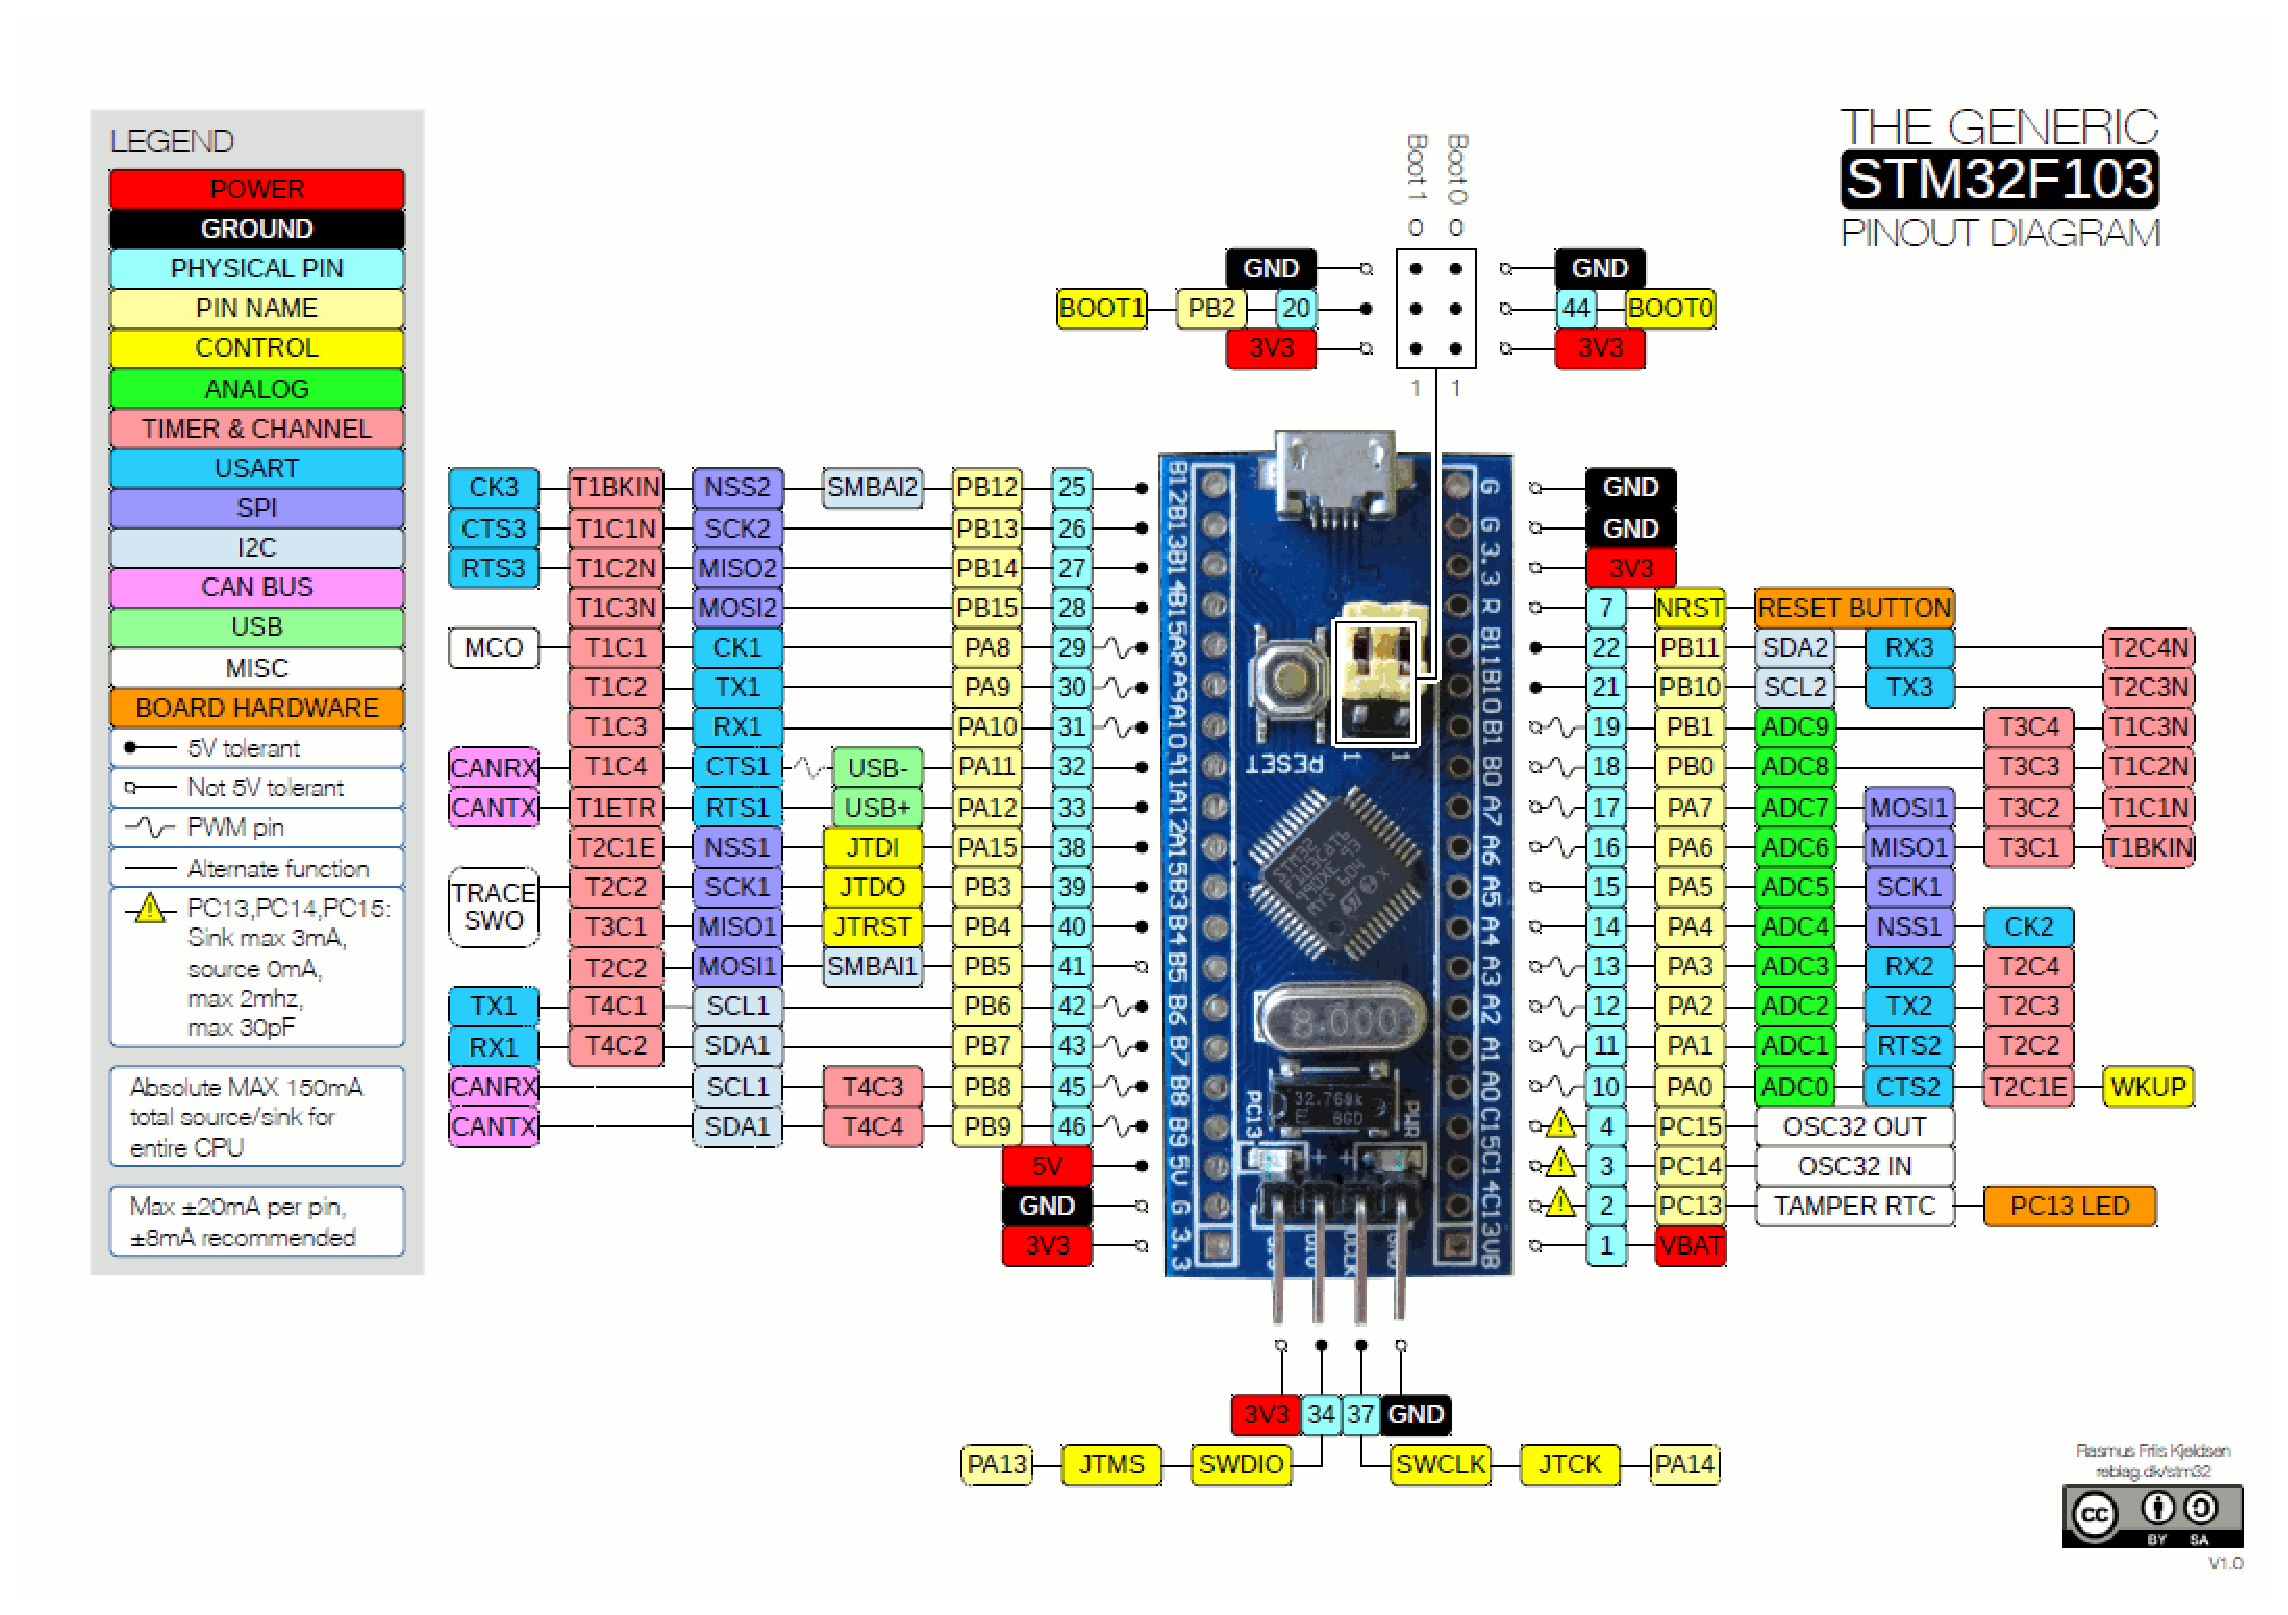
\includegraphics[width=\columnwidth]{./figs/stm_blue.eps}
\caption{STM32F103C8T6 Pin Configuration (Blue Pill)}
\label{fig:stm_blue}
\end{figure}
%

\section{Make File and Flashing}
\begin{enumerate}[1.]
\item Communicate with the STM32 board.  While using STLINK,
\begin{lstlisting}
cd ~/sandbox/openocd
sudo openocd -f /usr/local/share/openocd/scripts/interface/stlink.cfg -f usr/local/share/openocd/scripts/target/stm32f1x.cfg
\end{lstlisting}
If only RPI GPIO is used, then
\begin{lstlisting}
cd ~/sandbox/openocd
cp ~/sandbox/STM32F103C8T6/refs/openocd.cfg ~/sandbox/openocd
sudo openocd -f /usr/local/share/openocd/scripts/interface/sysfsgpio-raspberrypi.cfg -c 
"transport select swd" -c "adapter_khz 1000" -f /usr/local/share/openocd/scripts/target/stm32f1x.cfg
\end{lstlisting}
\item Open a new terminal and type
\begin{lstlisting}
telnet localhost 4444
\end{lstlisting}
This will establish a connection between the RPI and STM32
\item Open another new terminal and type
\begin{lstlisting}
cp ~/sandbox/STM32F103C8T6/examples/blink.c ~/sandbox/STM32F103C8T6/src/main.c
sudo make bin
cp main.bin cd ~/sandbox/openocd
\end{lstlisting}
Ensure that the following lines in the Makefile 
\begin{lstlisting}
CC= /data/data/com.termux/files/home/gcc-arm-none-eabi-8-2019-q3-update/install-native/bin/arm-none-eabi-gcc
OBJCOPY	= /data/data/com.termux/files/home/gcc-arm-none-eabi-8-2019-q3-update/install-native/bin/arm-none-eabi-objcopyOBJDUMP    = /data/data/com.termux/files/home/gcc-arm-none-eabi-8-2019-q3-update/install-native/bin/arm-none-eabi-objdump
/data/data/com.termux/files/home/gcc-arm-none-eabi-8-2019-q3-update/install-native/bin/arm-none-eabi-size $(PRJ_NAME).elf
\end{lstlisting}
%
are suitably modified based on the path in your OS.

%\item Make sure that the two pin caps (Boot0 and Boot1) beside the reset button are non-aligned.
\item Go to the telnet terminal 
\begin{lstlisting}
reset halt
flash write_image erase main.bin 0x08000000
reset run
\end{lstlisting}
\item Align the two pin caps beside the reset button. Press the reset button.  You should see an LED blinking.
\item Modify main.c in the STM32F103C8T6 directory and modify the code to keep the LED on. Flash it to the STM32 and verify.
%as
%\begin{lstlisting}
% while (1)
%  {
%    /* Turn on led connected to PC.4 pin */
%//    GPIO_SetBits(GPIOC, GPIO_Pin_13);
%    /* Insert delay */
%//    Delay(0xAFFFFF);
%
%    /* Turn off led connected to PC.4 pin */
%    GPIO_ResetBits(GPIOC, GPIO_Pin_13);
%    /* Insert delay */
%//   Delay(0xAFFFFF);
%  }
%\end{lstlisting}
%and flash the .bin file to the STM32.  What do you observe?
\end{enumerate}

\end{document}
